%% HEAD from knitr template
%% /Users/abarbour/Library/textemplates
%% Thu Feb  7 18:24:57 PST 2013
\documentclass[10pt]{article}\usepackage[]{graphicx}\usepackage[]{color}
%% maxwidth is the original width if it is less than linewidth
%% otherwise use linewidth (to make sure the graphics do not exceed the margin)
\makeatletter
\def\maxwidth{ %
  \ifdim\Gin@nat@width>\linewidth
    \linewidth
  \else
    \Gin@nat@width
  \fi
}
\makeatother

\definecolor{fgcolor}{rgb}{0.345, 0.345, 0.345}
\newcommand{\hlnum}[1]{\textcolor[rgb]{0.686,0.059,0.569}{#1}}%
\newcommand{\hlstr}[1]{\textcolor[rgb]{0.192,0.494,0.8}{#1}}%
\newcommand{\hlcom}[1]{\textcolor[rgb]{0.678,0.584,0.686}{\textit{#1}}}%
\newcommand{\hlopt}[1]{\textcolor[rgb]{0,0,0}{#1}}%
\newcommand{\hlstd}[1]{\textcolor[rgb]{0.345,0.345,0.345}{#1}}%
\newcommand{\hlkwa}[1]{\textcolor[rgb]{0.161,0.373,0.58}{\textbf{#1}}}%
\newcommand{\hlkwb}[1]{\textcolor[rgb]{0.69,0.353,0.396}{#1}}%
\newcommand{\hlkwc}[1]{\textcolor[rgb]{0.333,0.667,0.333}{#1}}%
\newcommand{\hlkwd}[1]{\textcolor[rgb]{0.737,0.353,0.396}{\textbf{#1}}}%

\usepackage{framed}
\makeatletter
\newenvironment{kframe}{%
 \def\at@end@of@kframe{}%
 \ifinner\ifhmode%
  \def\at@end@of@kframe{\end{minipage}}%
  \begin{minipage}{\columnwidth}%
 \fi\fi%
 \def\FrameCommand##1{\hskip\@totalleftmargin \hskip-\fboxsep
 \colorbox{shadecolor}{##1}\hskip-\fboxsep
     % There is no \\@totalrightmargin, so:
     \hskip-\linewidth \hskip-\@totalleftmargin \hskip\columnwidth}%
 \MakeFramed {\advance\hsize-\width
   \@totalleftmargin\z@ \linewidth\hsize
   \@setminipage}}%
 {\par\unskip\endMakeFramed%
 \at@end@of@kframe}
\makeatother

\definecolor{shadecolor}{rgb}{.97, .97, .97}
\definecolor{messagecolor}{rgb}{0, 0, 0}
\definecolor{warningcolor}{rgb}{1, 0, 1}
\definecolor{errorcolor}{rgb}{1, 0, 0}
\newenvironment{knitrout}{}{} % an empty environment to be redefined in TeX

\usepackage{alltt}
%%
%% !Rnw weave = knitr
%% sweave fig help:
%% http://users.stat.umn.edu/~geyer/Sweave/foo.pdf
%%
% \VignetteIndexEntry{ResponseModels}
% \VignetteEngine{knitr}
%
\usepackage{amsmath}
\usepackage{amssymb}
\usepackage[font=sf, labelfont={sf,bf}, margin=2cm]{caption}
\usepackage[T1]{fontenc}
\usepackage[utf8]{inputenc}
\usepackage{fancyvrb}
\usepackage{float}
\usepackage{geometry}
\geometry{verbose,tmargin=3cm,bmargin=5cm,lmargin=2.5cm,rmargin=2.5cm}
\usepackage{graphicx}
\usepackage{grffile}
\usepackage[pdfborder={0 0 0}]{hyperref}
\usepackage[utf8]{inputenc}
\usepackage{natbib}
\usepackage{makeidx}
\makeindex % comment to have no index
\usepackage{upquote}
\usepackage{url}
%
\author{Andrew J. Barbour}
\title{Demonstration of Well Response Functions}
\IfFileExists{upquote.sty}{\usepackage{upquote}}{}
\begin{document}
\maketitle
%\tableofcontents
%% BODY from knitr template
%\newcommand{\newcomm}[1]{#1}
%\renewcommand{\newcomm}[1]{#1}
%
\newcommand{\SC}[1]{\textsc{#1}}
\newcommand{\Rcmd}[1]{\texttt{#1}}
\newcommand{\bidxa}[1]{\index{#1}{\textbf{#1}}} 
\newcommand{\bidxb}[2]{\index{#2}{\textbf{#1}}} 
\newcommand{\idxa}[1]{\index{#1}{#1}} 
\newcommand{\idxb}[2]{\index{#2}{#1}} 
%
\begin{abstract}
abstract text
\end{abstract}
%
\section{Introduction}
Load the packages
\begin{knitrout}
\definecolor{shadecolor}{rgb}{0.969, 0.969, 0.969}\color{fgcolor}\begin{kframe}
\begin{alltt}
\hlkwd{library}\hlstd{(signal,} \hlkwc{warn.conflicts} \hlstd{=} \hlnum{FALSE}\hlstd{)}
\end{alltt}


{\ttfamily\noindent\itshape\color{messagecolor}{\#\# Loading required package: MASS}}\begin{alltt}
\hlkwd{library}\hlstd{(kitagawa,} \hlkwc{warn.conflicts} \hlstd{=} \hlnum{FALSE}\hlstd{)}
\end{alltt}


{\ttfamily\noindent\itshape\color{messagecolor}{\#\# Loading required package: kelvin\\\#\# Loading required package: Bessel\\\#\# Loading required package: Rmpfr\\\#\# Loading required package: gmp\\\#\# \\\#\# Attaching package: 'gmp'\\\#\# \\\#\# The following object is masked from 'package:base':\\\#\# \\\#\#\ \ \ \  \%*\%, apply, crossprod, matrix, tcrossprod}}\begin{verbatim}
## Loading C code of R package 'Rmpfr': GMP using 64 bits per limb
\end{verbatim}


{\ttfamily\noindent\itshape\color{messagecolor}{\#\# \\\#\# Attaching package: 'Rmpfr'\\\#\# \\\#\# The following object is masked from 'package:stats':\\\#\# \\\#\#\ \ \ \  pnorm, print.integrate\\\#\# \\\#\# The following object is masked from 'package:base':\\\#\# \\\#\#\ \ \ \  cbind, pmax, pmin, rbind\\\#\# \\\#\# Loaded kelvin (1.2.2) -- Solutions to the Kelvin differential equation.\\\#\# Loaded kitagawa (2.0.2) -- Spectral response of water wells}}\end{kframe}
\end{knitrout}


\section{Sealed well response}
\subsection{Strain: Kitagawa (2011)}
%
\citet{kitagawa2011}

\section{Open well response}
\subsection{Strain: Rojstaczer (1988)}
%
\citet{rojstaczer1988, rojstaczer1988b}

\begin{knitrout}
\definecolor{shadecolor}{rgb}{0.969, 0.969, 0.969}\color{fgcolor}\begin{kframe}
\begin{alltt}
\hlcom{# Some dummy parameters}
\hlstd{z} \hlkwb{<-} \hlnum{1}
\hlstd{Trans} \hlkwb{<-} \hlnum{1}
\hlstd{Stor} \hlkwb{<-} \hlnum{1}
\hlstd{Diffus} \hlkwb{<-} \hlstd{Trans}\hlopt{/}\hlstd{Stor}
\hlcom{# Nondimensional frequencies}
\hlstd{Q} \hlkwb{<-} \hlnum{10}\hlopt{^}\hlkwd{seq}\hlstd{(}\hlopt{-}\hlnum{3}\hlstd{,} \hlnum{2}\hlstd{,} \hlkwc{by} \hlstd{=} \hlnum{0.1}\hlstd{)}  \hlcom{# == z**2 omega / 2 D}
\hlstd{omega} \hlkwb{<-} \hlkwd{omega_norm}\hlstd{(Q, z, Diffus,} \hlkwc{invert} \hlstd{=} \hlnum{TRUE}\hlstd{)}  \hlcom{# == Q * 2 * Diffus / z**2}
\hlstd{wrsp} \hlkwb{<-} \hlkwd{open_well_response}\hlstd{(omega,} \hlkwc{T.} \hlstd{= Trans,} \hlkwc{S.} \hlstd{= Stor,} \hlkwc{z.} \hlstd{= z,} \hlkwc{model} \hlstd{=} \hlstr{"rojstaczer"}\hlstd{,}
    \hlkwc{as.pressure} \hlstd{=} \hlnum{FALSE}\hlstd{)}
\hlstd{crsp} \hlkwb{<-} \hlstd{wrsp[,} \hlnum{2}\hlstd{]}
\hlcom{# }
\hlstd{lQ} \hlkwb{<-} \hlkwd{log10}\hlstd{(Q)}
\hlcom{# Amplitude}
\hlstd{As} \hlkwb{<-} \hlnum{0.05}  \hlcom{# cm/nE}
\hlstd{Gain} \hlkwb{<-} \hlkwd{Mod}\hlstd{(crsp)}
\hlcom{# Phase}
\hlstd{Phs} \hlkwb{<-} \hlkwd{Arg}\hlstd{(crsp)}  \hlcom{# will wrap to -pi/pi}
\hlstd{uPhs} \hlkwb{<-} \hlstd{signal::}\hlkwd{unwrap}\hlstd{(Phs,} \hlkwc{tol} \hlstd{= pi}\hlopt{/}\hlnum{30}\hlstd{)}
\end{alltt}
\end{kframe}
\end{knitrout}


\begin{figure}[htb!]
\begin{center}
\begin{knitrout}
\definecolor{shadecolor}{rgb}{0.969, 0.969, 0.969}\color{fgcolor}
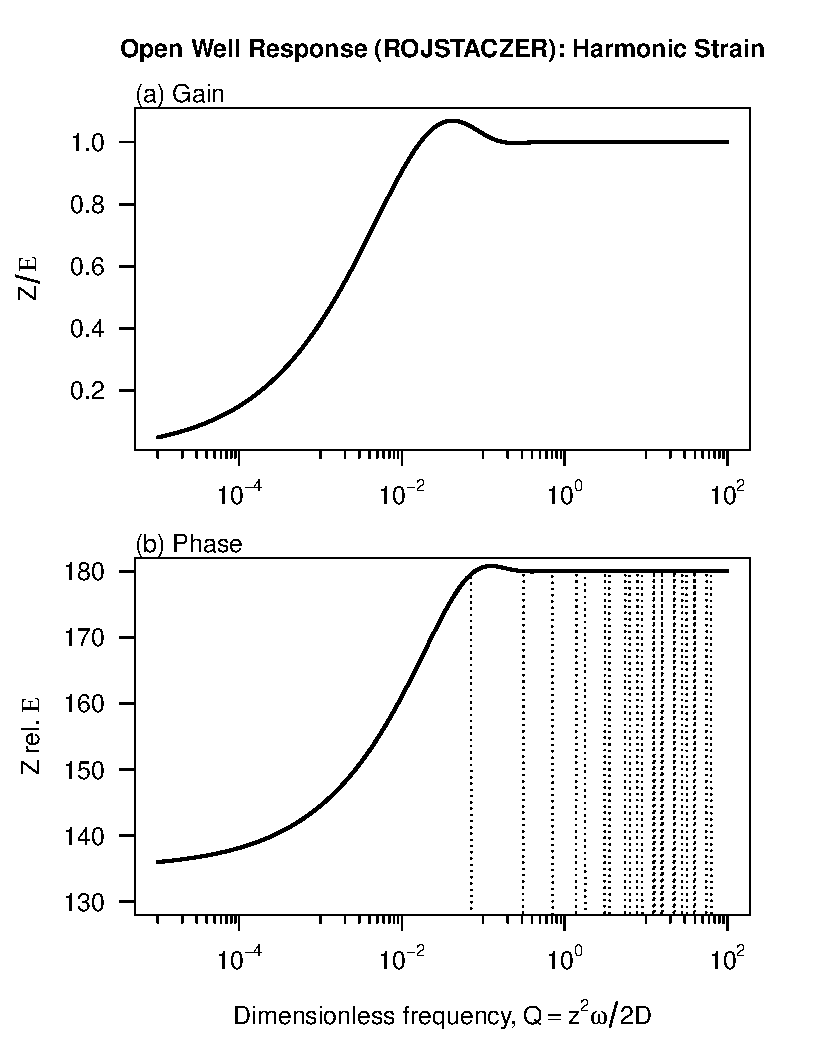
\includegraphics[width=\maxwidth]{figure/ROJRESPFIG} 

\end{knitrout}

\caption{The response of an open well to harmonic areal strain using
the Rojstaczer model. Modified from \citet[][Fig.~3]{rojstaczer1988}.
Frequency is dimensionless, based on the well-depth $z$ and the diffusivity
$D$.}
\label{fig:tmp}
\end{center}
\end{figure}

%% TAIL from knitr template
\bibliographystyle{apalike}
\bibliography{REFS}

\printindex

\end{document}
